\documentclass[final,hyperref={pdfpagelabels=false}, professionalmath, mathserif, 11pt]{beamer}
\usepackage{grffile}
\mode<presentation>{\usetheme{BGC_retreat}}
\usepackage[english]{babel}
\usepackage[utf8]{inputenc}
\usepackage{sidecap}
\usepackage{natbib}


\def\mytitle{Code for the comunity I: working at the site level}
\def\myauthor{Department Biogeochemical Integration\vspace{1cm}}
%M.~Forkel\quad
%F.~Gans\quad
%M.D.~Mahecha\quad
%M.~Migliavacca\quad
%A.~Moffat\\
%M.~Reichstein\quad
%O.~P{\'e}rez\quad
%J.~v.~Buttlar\quad
%T.~Wutzler
%}


\usepackage{setspace}
\setstretch{1.25}



%%%%%%%%%%%%%%%%%%%%%%%%%%%%%%%%%%%%%%%%%%%%%%%%%%%%%%%%%%%%%%%%%%%%%%%%%%%%%%%%%%%%%%
\begin{document}
\begin{frame}
\vspace{3ex}
\begin{columns}
\begin{column}{.48\textwidth}
\begin{center}
\begin{minipage}[T]{.95\textwidth}
\parbox[t][\columnheight]{\textwidth}{

\begin{block}{\vspace{.2cm}\textbf{REddyProc}\hfill\normalsize{A. Moffat, T. Wutzler, O. Menzer \& M. Migliavacca}}
\alert{\textit{Context:}}
\begin{itemize}
    \item Data from eddy covariance measurements are key to understand atmosphere ecosystem exchange fluxes.
    \item A standardized processing of the raw data is necessary to ensure comparability across sites.
    \item Site PIs will benefit from being able to process their data by using the easy-to-use R-package.
\end{itemize}
 
\alert{\textit{Methods provided:}}
\begin{itemize}
    \item Filling gaps in the time series and providing uncertainties for the estimates.
    \item Partitioning net flux NEE into gross fluxes GPP and respiration.
    \item Filtering for unfavourable conditions of low turbulance (u-Star filtering, in test phase).
\end{itemize}
\vspace{1cm}

\begin{columns}
\column{.8\textwidth}
    \begin{figure}[tb]
    \begin{center}
        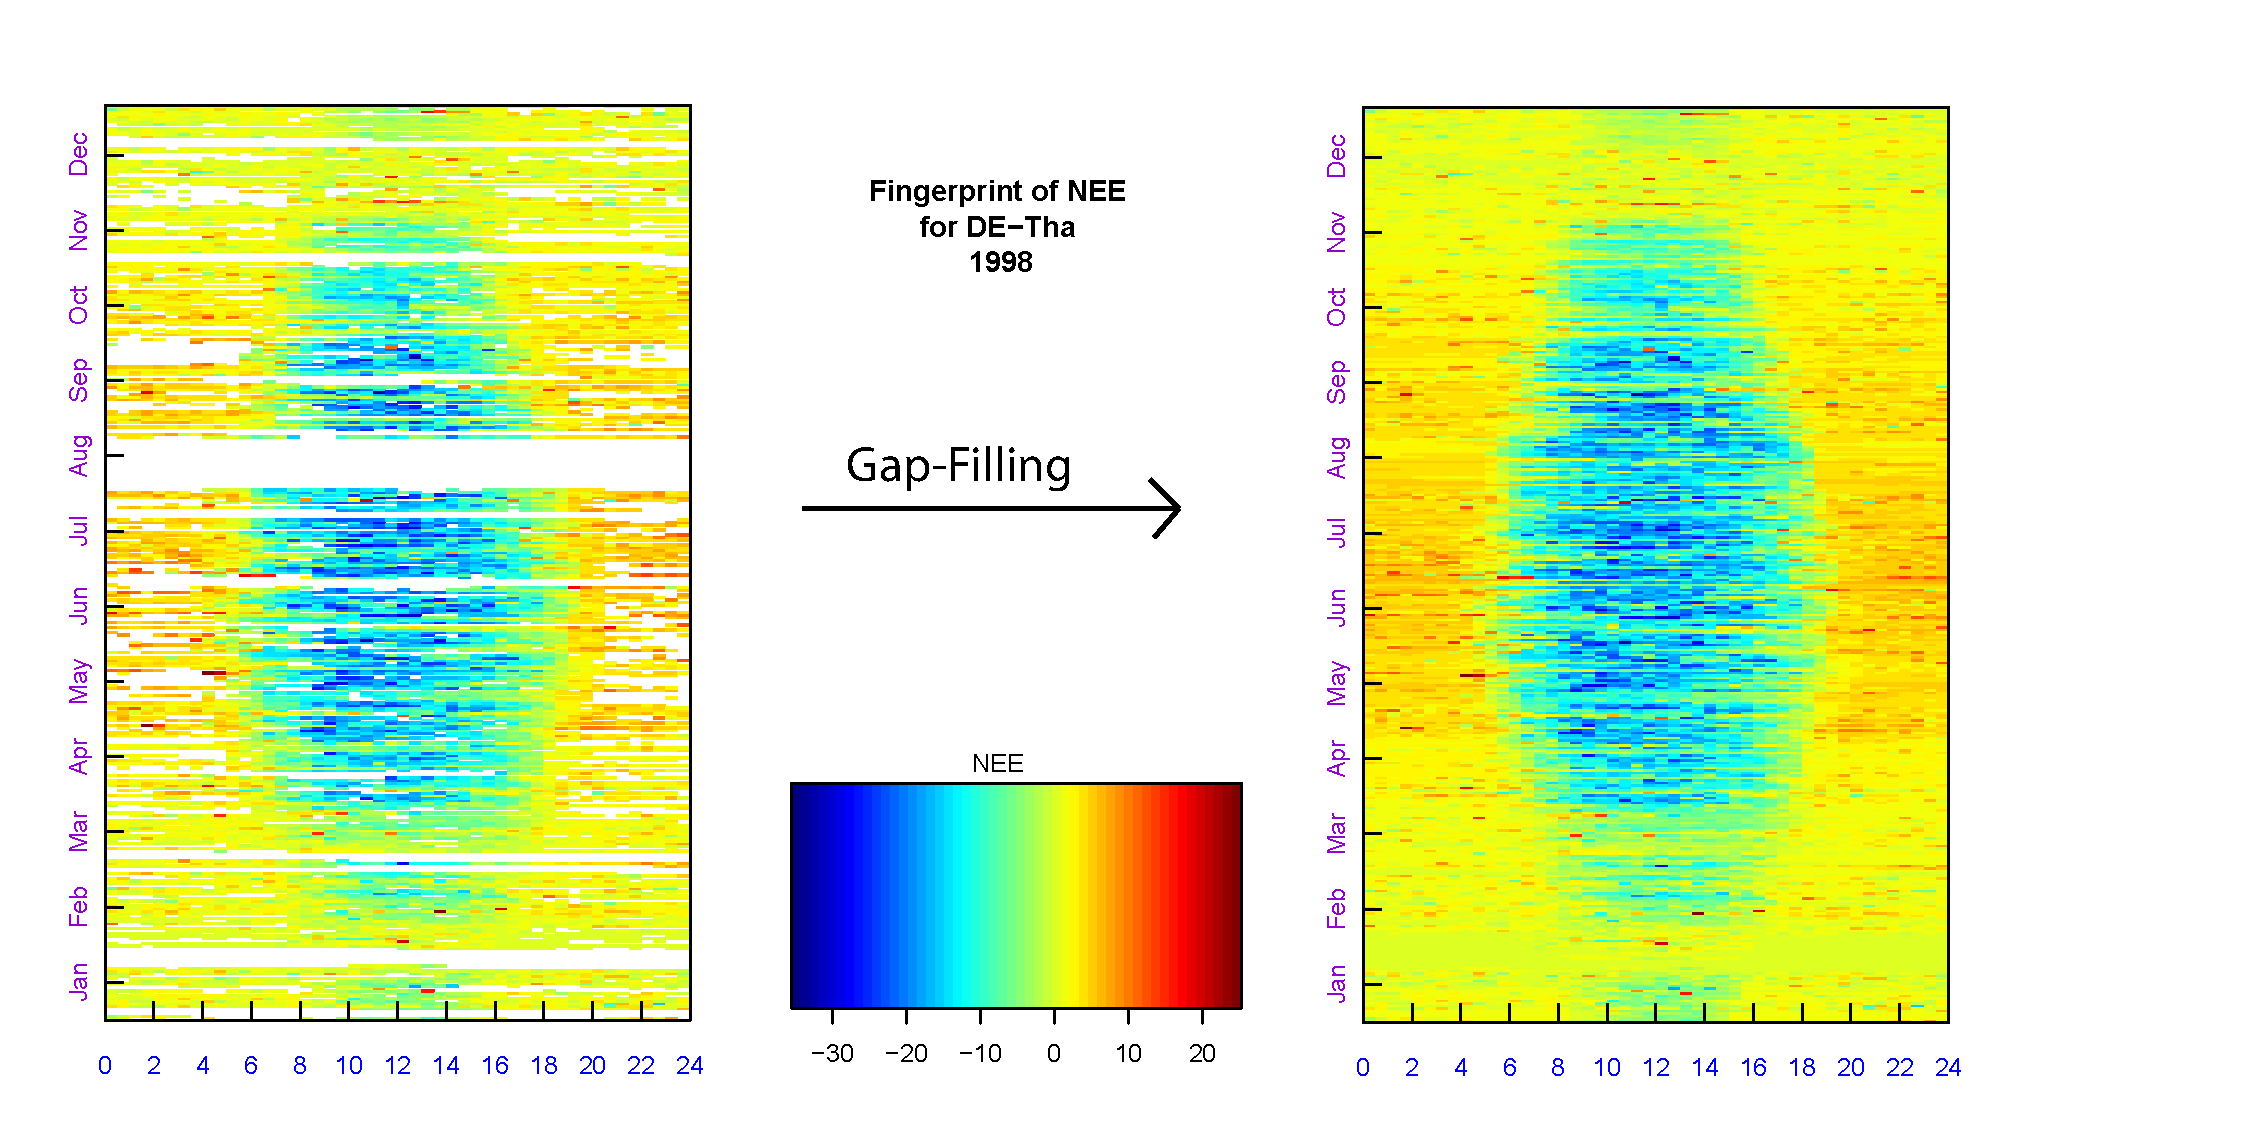
\includegraphics[width=.95\textwidth]{DE-Tha_1998_FP_NEE_ffc}
    \end{center}
    \end{figure}
\column{.2\textwidth}
\small{\textit{A fingerprint of ecosystem: Net ecosystem exchange (NEE) versus daytime and yearday}}
\vspace{4cm}
	\begin{figure}[tb]
		
\includegraphics[width=.6\textwidth]{qrcodeREddyProc.jpg}
	\end{figure}
\end{columns}
\vspace{1cm}
\hfill\large{\url{https://www.bgc-jena.mpg.de/bgi/index.php/Services/REddyProcWeb}}
\end{block}
\vspace{3ex}

\begin{block}{\textbf{RSCAPE}\hfill\normalsize{F. Gans \& M.D. Mahecha}}
\alert{\textit{Context:}}
\begin{itemize}
	\item Temperature is a key control of biogeochemical processes (e.g. on CO$_2$, CH$_4$, or N$_2$O production rates in soils)
.
	\item On seasonal and longer timescales other ecological factors e.g. substrate availability play an important role.
	\item The interaction of processes on different timescales is complicating the estimation of the temperature sensitivity of biogeochemcial processes.
\end{itemize}
 
\alert{\textit{Methods provided:}}
\begin{itemize}
	\item RSCAPE implements the "scale dependent parameter estimation” (SCAPE) principle \citep{MAHECHAetal2010b}.
    \item The user can choose amongst a wide range of 1) spectral decomposition methods and 2) standard or custom temperature sensitivity models.
    \item Full consideration to time-lagged responses and methodologcical uncertainties.
\end{itemize}
\vspace{1cm}
\begin{columns}
\column{.8\textwidth}
	\begin{figure}[tb]
	\begin{center}
		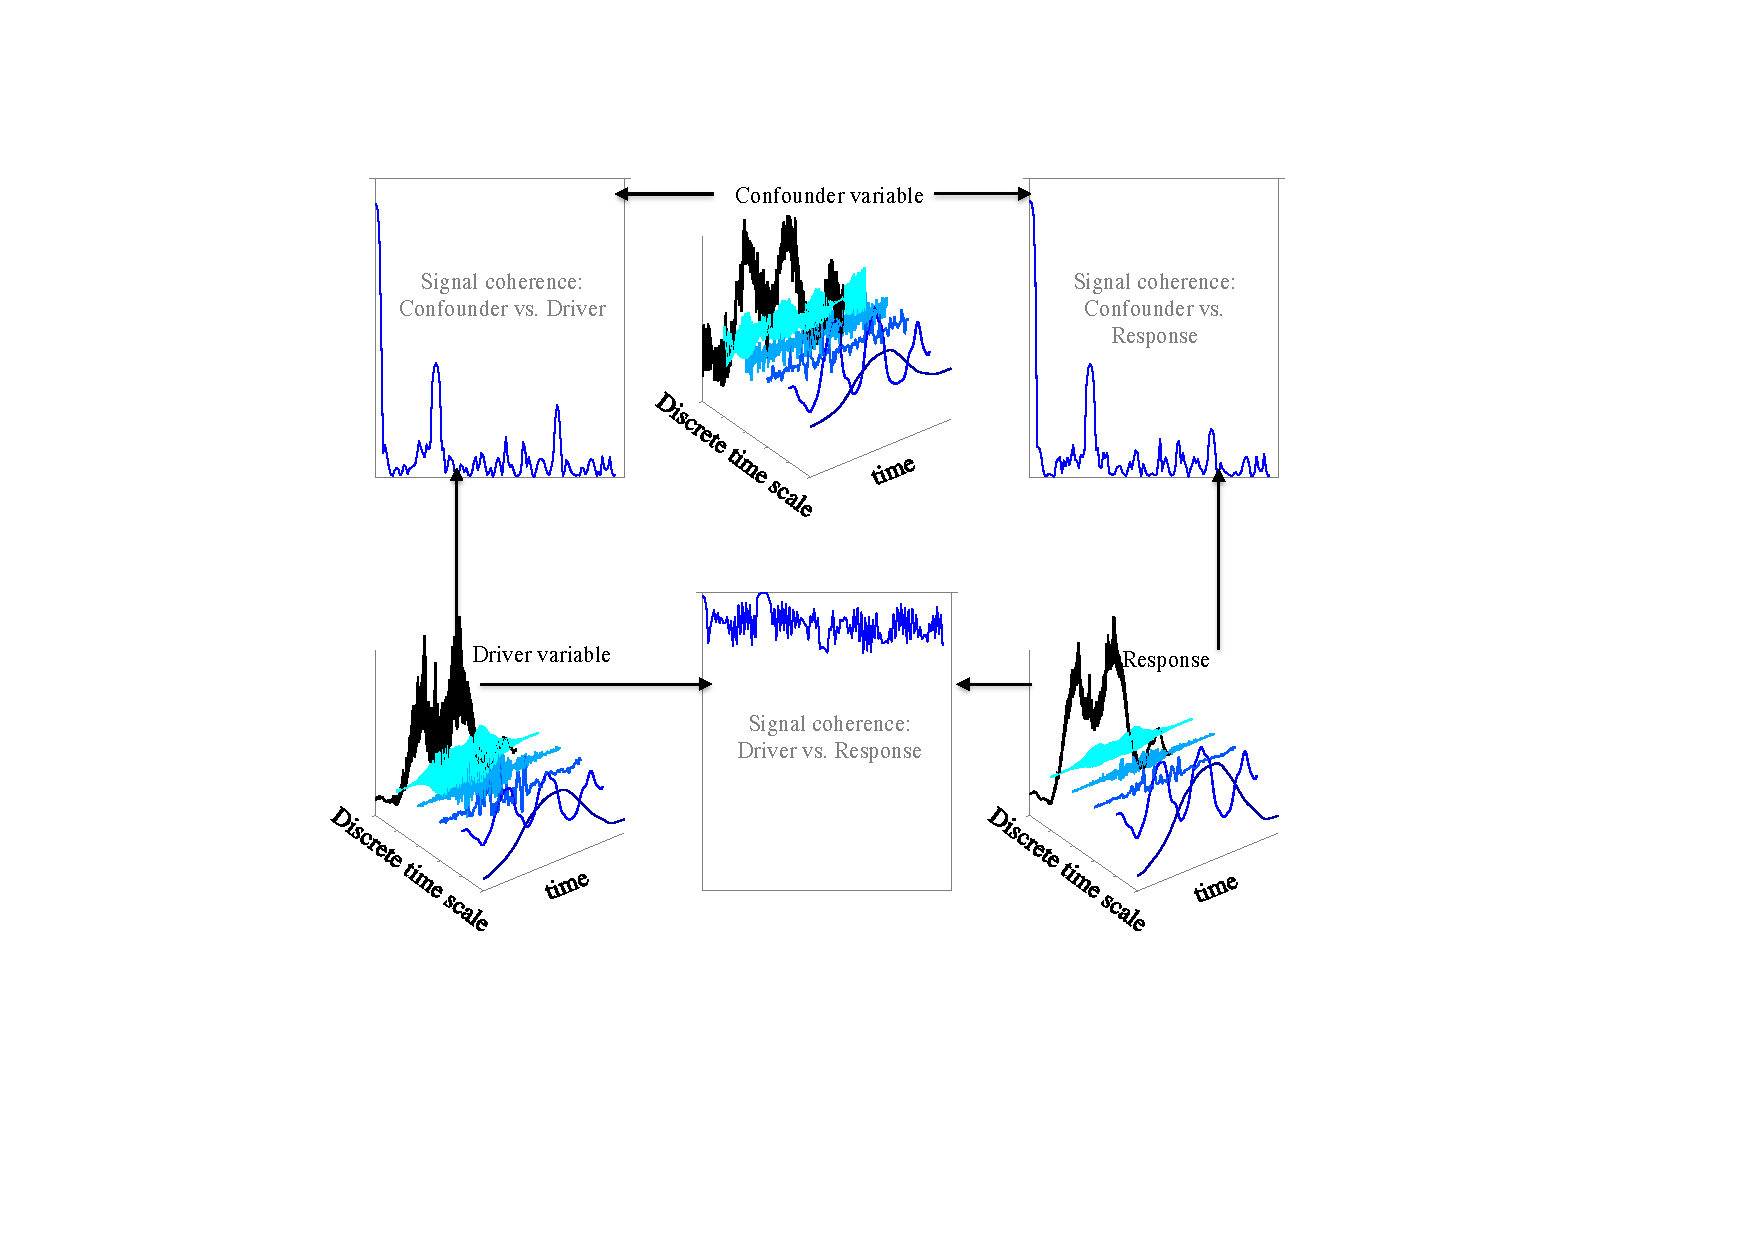
\includegraphics[width=.95\textwidth]{FIG1.pdf}
	\end{center}
	\end{figure}
\column{.2\textwidth}
\small{\textit{Conceptual problem solved by RSCAPE: The parameter estimtation problem (mapping from driver to response) is confounded on different time scales}}
\vspace{4cm}
	\begin{figure}[tb]
		
\includegraphics[width=.6\textwidth]{qrcode-RSCAPE.jpg}
	\end{figure}
\end{columns}
\vspace{1cm}
\hfill\large{\url{https://github.com/meggart/RSCAPE}}
\end{block}


\vfill

}

         
			          
\end{minipage}
\end{center}
\end{column}    








% -------------
% SECOND COLUMN
% -------------



\begin{column}{.48\textwidth}
\begin{minipage}[T]{.95\textwidth}
\parbox[t][\columnheight]{\textwidth}{}
\end{minipage}
\end{column}   
\end{columns}

\bibliographystyle{apalike}
\bibliography{/Users/mmahecha/manuscripts/MahechaBIBTEX2014}

\end{frame}
\end{document}
